\section*{Introdução}

\paragraph{Definição.} A \textbf{Matemática Discreta} manipula objetos \textbf{contáveis}
utilizando sistemas matemáticos adequados para cada tipo de problema.
Exemplo: números inteiros.

Algumas aplicações da Matemática Discreta

\begin{itemize}
\item
  Métodos formais para especificação, verificação e validação de
  software;
\item
  Análise da complexidade dos algoritmos;
\item
  Algoritmos combinatórios: grafos, expressões booleanas, \(\dots\);
\item
  Probablidade;
\item
  Computabilidade;
\item
  Cálculo numérico;
\item
  Criptografia
\item
  \(\dots\)
\end{itemize}

    \hypertarget{alguns-sistemas-matemuxe1ticos-discretos}{%
\subsection*{Alguns Sistemas Matemáticos
Discretos}\label{alguns-sistemas-matemuxe1ticos-discretos}}

\begin{itemize}
\item
  Lógica
\item
  Teoria dos Conjuntos
\item
  Teoria dos Números
\item
  Análise Combinatória
\item
  Teoria dos Grafos
\end{itemize}

\end{document}

    \hypertarget{nouxe7uxf5es-de-luxf3gica}{%
\subsection{Noções de Lógica}\label{nouxe7uxf5es-de-luxf3gica}}

\hypertarget{axioma-ou-postulado}{%
\subsubsection{Axioma ou Postulado}\label{axioma-ou-postulado}}

\emph{Axioma} é uma premissa ou ponto de partida para o raciocínio. É
tão evidente que é aceito como verdadeiro sem controvérsia e sem
necessidade de prova.

Exemplo: Axioma de Peano para as propriedades dos números naturais.

\begin{enumerate}
\def\labelenumi{\arabic{enumi}.}
\item
  \(0 \in Nat\)
\item
  \(x=x\)
\item
  \(x=y \Rightarrow y=x\)
\item
  \(x=y\wedge y=z\Rightarrow x=z\)
\end{enumerate}

    \hypertarget{teorema}{%
\subsubsection{Teorema}\label{teorema}}

\textbf{Teorema} é uma afirmação cuja veracidade pode ser demonstrada
utilizando operações e argumentos matemáticos aceitáveis.

    \begin{center}
	    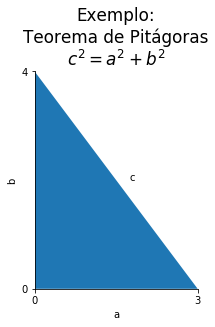
\includegraphics[scale=.6]{img/pitagoras.png}
    \end{center}
    { \hspace*{\fill} \\}
    
    \hypertarget{termos-adicionais}{%
\subsubsection{Termos adicionais}\label{termos-adicionais}}

\begin{itemize}
\item
  \textbf{Definição} especifica o significado de palavra ou frase em
  utilizando conceitos já conhecidos. Também é aceita sem prova.
\item
  \textbf{Proposição} é um termo genérico para um teorema sem
  importância particular. Este termo denota um afirmação que exige um
  prova simples, enquanto \emph{teorema} é reservado para resultados de
  maior importância com prova difícil ou longa.
\item
  \textbf{Lema} é uma \emph{proposição} que faz parte da prova de um
  teorema por possuir pouca aplicabilidade.
\item
  \textbf{Corolário} é uma \emph{proposição} que segue com pouca ou
  nenhuma prova, outra definição ou teorema.
\end{itemize}

